\documentclass[11pt,a4paper]{report}
\usepackage{lipsum}
\usepackage{style_bpifrance}
%------------------Document----------------------------

\begin{document}

\titre{Document de Méthodologie du Modèle de Pilotage des fonds de garantie individuels}

\tableofcontents


\newpage
\part{Introduction et problématique de modélisation}

\chapter{Etapes de la simulation du passif d'un fonds de garantie}
\section{Section}

Lorem ipsum dolor sit amet, consectetur adipiscing elit. Donec nec fermentum augue. Integer id neque sit amet augue lacinia fringilla. Donec leo ipsum, dapibus vel orci et, viverra viverra sem. Morbi maximus neque ipsum, in vulputate libero porta a. Interdum et malesuada fames ac ante ipsum primis in faucibus. Nulla at libero arcu. 
o ipsum, dapibus vel orci et, viverra viverra sem. Morbi maximus neque ipsum, in vulputate libero porta a. Interdum et malesuada fames ac ante ipsum primis in faucibus. Nulla at libero arcu. 


\section{Second Section}

\[
\boxedb{\int_{-\infty}^{+\infty} e^{-x^2/2}dx = \sqrt{2\pi}.}
\]

\[
\boxedb{Z_{i,j,t} = -\sqrt{\rho_j}X_t + \sqrt{1-\rho_j}\varepsilon_{i,j,t}}
\]

De plus, les taux de sinistralités sont modélisés par :
\[
S_{i,j,t} = H^{-1}_{\mu,\sigma}(\Phi(Z_{i,j,t}))
\]


\begin{figure}[htb]
\centering
  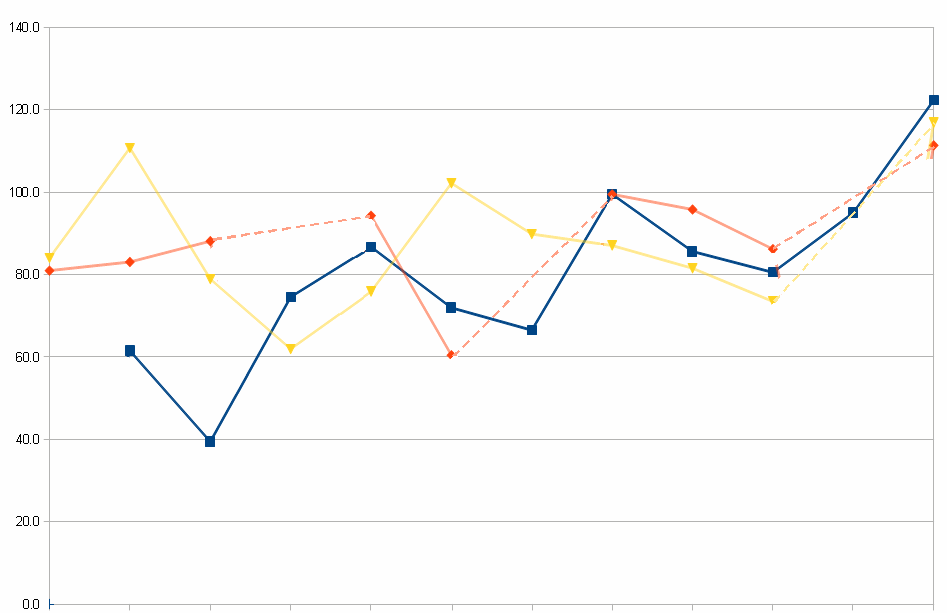
\includegraphics[width=1\textwidth]{figures/figure1.png}
 \centering
  {\textbf{\caption{Figure Description}}}\label{fig:1}
\end{figure}


\subsection{Subsection}

In pretium enim dui, quis ornare odio varius et. Nulla facilisi. Nunc tristique tortor at urna vehicula, elementum bibendum tortor hendrerit. Ut eu risus nisi. Vestibulum nunc lorem, tristique sed ultrices nec, porta et ligula. Nam facilisis felis a congue auctor. Fusce id odio in libero blandit cursus nec nec arcu. Nulla eu ultricies massa, id dapibus nisi. Donec tellus urna, maximus nec semper id, consectetur eu mi. Vestibulum elit eros, porta ac eros a, mattis pulvinar magna. Nulla pellentesque dapibus leo molestie varius. Duis ut rutrum urna, at condimentum dui. Sed orci magna, faucibus nec quam et, malesuada ultrices velit. Nam a lorem a massa facilisis rutrum eget id nunc. Morbi aliquet felis et tincidunt scelerisque. 

\subsubsection{Subsubsection}
\lipsum

\begin{itemize}
    \item test
    \item testing
\item tester
\end{itemize}

\paragraph{Etape 1 : Simulation de la trajectoire future du facteur de risque systémique $Y_t$}
On utilise le modèle de dynamique pour $Y_t$ pour simuler différentes trajectoires futures $Y_t$  du facteur de risque jusqu’à la maturité résiduelle maximale des concours garantis. 

\subsubsection{Autre subsubsection}
Chaque valeur du facteur de risque est commune à toutes les entreprises

% %-------------------------Content------------------------
\subsection{Testing another subsection}

In pretium enim dui, quis ornare odio varius et. Nulla facilisi. Nunc tristique tortor at urna vehicula, elementum bibendum tortor hendrerit. Ut eu risus nisi. Vestibulum nunc lorem, tristique sed ultrices nec, porta et ligula. Nam facilisis felis a congue auctor. Fusce id odio in libero blandit cursus nec nec arcu. Nulla eu ultricies massa, id dapibus nisi. Donec tellus urna, maximus nec semper id, consectetur eu mi. Vestibulum elit eros, porta ac eros a, mattis pulvinar magna. Nulla pellentesque dapibus leo molestie varius. Duis ut rutrum urna, at condimentum dui. Sed orci magna, faucibus nec quam et, malesuada ultrices velit. Nam a lorem a massa facilisis rutrum eget id nunc. Morbi aliquet felis et tincidunt scelerisque. 

\paragraph{Lecture du tableau :} 
Prenons l’exemple du fonds de garantie Création et le cas des simulations au 30/06/2018. Notons par « S » le semestre de simulation (le 1er semestre 2018). Les montants utilisés par génération d’autorisation doivent être multipliés par :
\begin{itemize}
    \item 1.222 pour les autorisations du semestre « $S$ », c’est-à-dire de délai égal à 0 ;
    \item 1.047 pour les autorisations du semestre « $S -1$ », c’est-à-dire de délai égal à 1 ;
    \item 1.023 pour les autorisations du semestre « $S-2$ », c’est-à-dire de délai égal à 2.
\end{itemize}

\paragraph{}
In pretium enim dui, quis ornare odio varius et. Nulla facilisi. Nunc tristique tortor at urna vehicula, elementum bibendum tortor hendrerit. Ut eu risus nisi. Vestibulum nunc lorem, tristique sed ultrices nec, porta et ligula. Nam facilisis felis a congue auctor. Fusce id odio in libero blandit cursus nec nec arcu. Nulla eu ultricies massa, id dapibus nisi. Donec tellus urna, maximus nec semper id, consectetur eu mi.

\paragraph{Quelques remarques :}
\begin{itemize}
    \item La première méthode a principalement deux inconvénients :
    \begin{itemize}
        \item Le choix de la loi de probabilité est purement statistique. Elle ne se base sur aucune connaissance a priori du phénomène.
        \item La méthode ne garantit pas le choix d’une loi de probabilité qui modélise bien la queue de distribution. Or dans la modélisation quantitative du risque, la queue de distribution est très importante.
    \end{itemize}
    \item La deuxième méthode présente également quelques inconvénients : la loi choisie n’est pas statistiquement la loi la plus proche au vu des données historiques. Comment justifier le choix d’une loi plutôt qu’une autre ?
    \item Blabla
\end{itemize}

\section{Taux d'utilisation}

\newpage

\chapter{Formalisation}
Exprimons le problème qui nous intéresse sous le format d'un problème d'optimisation de programmation linéaire.

\section{Variables}

\begin{itemize}\itemsep2pt
    \item $z$ : année observée
    \item $( i , j )$ : années de (début,fin) d'un swap forward
    \item $N_0$ : Nominal constant (celui du swap à répliquer)
    \item $s_{i,j}$ : taux du swap forward débutant dans i années et finissant dans j (à partir d'aujourd'hui)
    \item $N_{i,j}$ : Nominal du swap forward débutant dans i années et finissant dans j (à partir d'aujourd'hui)
    \item $D_{i,j}$ : Duration du swap forward débutant dans i années et finissant dans j (à partir d'aujourd'hui)
    \item $c_z$ : coupon reçu à l'année $z$
    \item $x_z$ : plafond du coupon fixe reçu à l'année $z$
\end{itemize}

Il est à noter que la matrice $s$ est celle de la Figure 4. 

La matrice (puis plus tard le vecteur) à optimiser est la matrice des $N_{i,j}$. Son état initial est :  
\begin{itemize}\itemsep2pt
    \item $N_0$ en $(0,n) $
    \item 0 partout ailleurs
\end{itemize}


\section{Fonction Objectif}


%$$\min_{N_{i,j}} \left | \sum_{i,j} ( N_{i,j} \cdot  D_{i,j} ) - N_0 \cdot D_{0,n} \ \right | $$

\[ \max_{N_{i,j}}  \sum_{i,j} ( N_{i,j} \cdot  s_{i,j} )  \]


Cela correspond à minimiser l'écart entre la couverture du portefeuille de swaps forwards et celle du swap initial.  Cette fonction objectif incite donc, toute autre contrainte par ailleurs, à  traiter peu de swaps et avec la maturité la plus longue possible.

\subsection{Contraintes}

\begin{enumerate}
%   \item $ \forall z \in [|1,n|],\quad \ c_z = \sum\limits_{j \geq z , i < z} s_{i,j} N_{i,j} $  \qquad \qquad (valeur du coupon)
    \item $ \forall i,j  \qquad \qquad \qquad  N_{i,j} \geq 0 $ \qquad \qquad \qquad  \qquad (swaps receveurs uniquement)
    \item $ \forall j   \qquad \qquad \qquad i \geq j  \Rightarrow \  N_{i,j} = 0 $ \quad \qquad  \qquad (swaps plausibles uniquement)
    \item $ \forall z \in [|1,n|], \quad N_0 = \sum\limits_{i < z} N_{Col_i} - \sum\limits_{j < z} N_{Row_j}  $ \quad (nominal constant)
    \item $ \forall z \in [|1,n|], \quad c_z \leq x_z  $  \qquad  \qquad  \qquad  \qquad  \qquad (pilotage de la MNI)
\end{enumerate}



\end{document}
